


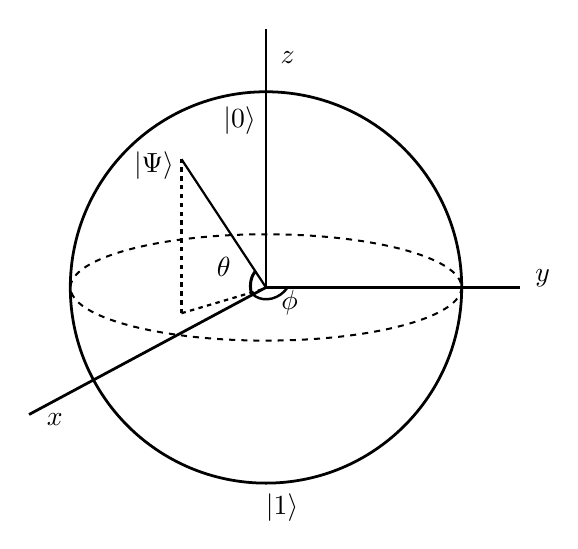
\begin{tikzpicture}[y=0.80pt, x=0.8pt,yscale=-1, inner sep=0pt, outer sep=0pt]
% path2991
\path[shift={(122.78385,63.61424)},draw=black,miter limit=4.00,line
  width=1.000pt] (377.7970,266.9686) .. controls (377.7970,315.7841) and
  (338.2242,355.3569) .. (289.4087,355.3569) .. controls (240.5931,355.3569) and
  (201.0203,315.7841) .. (201.0203,266.9686) .. controls (201.0203,218.1530) and
  (240.5931,178.5802) .. (289.4087,178.5802) .. controls (338.2242,178.5802) and
  (377.7970,218.1530) .. (377.7970,266.9686) -- cycle;

% path2993
\path[cm={{1.41275,0.0,0.0,1.33158,(-12.64299,-20.43742)}},draw=black,dash
  pattern=on 2.19pt off 2.19pt,miter limit=4.00,line width=0.729pt]
  (363.2143,263.6122) .. controls (363.2143,273.5730) and (335.2321,281.6479) ..
  (300.7143,281.6479) .. controls (266.1965,281.6479) and (238.2143,273.5730) ..
  (238.2143,263.6122) .. controls (238.2143,253.6513) and (266.1965,245.5765) ..
  (300.7143,245.5765) .. controls (335.2321,245.5765) and (363.2143,253.6513) ..
  (363.2143,263.6122) -- cycle;

% path3767
\path[draw=black,line join=miter,line cap=butt,miter limit=4.00,line
  width=1.000pt] (412.1925,213.8787) .. controls (412.1925,213.8787) and
  (412.1925,213.8787) .. (412.1925,330.5828) .. controls (526.6869,330.5828) and
  (526.6869,330.5828) .. (526.6869,330.5828);

% path3769
\path[draw=black,line join=miter,line cap=butt,miter limit=4.00,line
  width=1.000pt] (412.1813,330.5940) .. controls (305.1728,387.9706) and
  (305.1728,387.9706) .. (305.1728,387.9706);

% path4771
\path[draw=black,line join=miter,line cap=butt,line width=0.800pt]
  (412.1925,330.5827) .. controls (374.0142,272.6528) and (374.0142,272.6528) ..
  (374.0142,272.6528);

% path4773
\path[draw=black,dash pattern=on 1.60pt off 1.60pt,line join=miter,line
  cap=butt,miter limit=4.00,line width=0.800pt] (374.0142,342.3220) --
  (374.0142,272.7624);

% path4773-4
\path[draw=black,dash pattern=on 1.60pt off 1.60pt,line join=miter,line
  cap=butt,miter limit=4.00,line width=0.800pt] (374.0142,342.2321) --
  (411.6925,331.0830);

% path5193
\path[cm={{0.78149,0.0,0.0,1.07444,(348.5525,74.37157)}},draw=black,line
  join=bevel,miter limit=4.00,line width=1.091pt] (72.8896,240.5759) .. controls
  (71.7870,237.3261) and (72.7735,233.7325) .. (75.3807,231.5011);

% path5193-1
\path[cm={{-0.58224,-0.78271,1.04136,-0.82723,(213.06085,585.73163)}},draw=black,line
  join=bevel,miter limit=4.00,line width=0.878pt] (71.5872,240.5323) .. controls
  (69.8535,236.2130) and (72.5902,231.5235) .. (77.6998,230.0580) .. controls
  (78.4960,229.8296) and (79.3237,229.6891) .. (80.1624,229.6399);

% text3455
\path[fill=black] (419.11932,343.09579) node[above right] (text3455) {$\phi$};

% text3455-7
\path[fill=black] (389.96484,325.63696) node[above right] (text3455-7)
  {$\theta$};

% text3455-0
\path[fill=black] (392.9953,261.41104) node[above right] (text3455-0)
  {$|0\rangle$};

% text3455-4
\path[fill=black] (418.75418,229.65216) node[above right] (text3455-4) {$z$};

% text3455-8
\path[fill=black] (533.91156,330.18265) node[above right] (text3455-8) {$y$};

% text3455-45
\path[fill=black] (352.5892,281.6344) node[above right] (text3455-45)
  {$|\Psi\rangle$};

% text3455-1
\path[fill=black] (313.19327,392.8121) node[above right] (text3455-1) {$x$};

% text3455-11
\path[fill=black] (412.1882,436.20804) node[above right] (text3455-11)
  {$|1\rangle$};


\end{tikzpicture}
